%%%%%%%%%%%%%%%%%%%%%%%%%%%%%%%%%%%%%%%%%%%%%%%%%%%%%%%%%%%%%%%%%%%%%%%%%%%%%%%
\section{Methodology}
\label{sec:methodology}
%%%%%%%%%%%%%%%%%%%%%%%%%%%%%%%%%%%%%%%%%%%%%%%%%%%%%%%%%%%%%%%%%%%%%%%%%%%%%%%

%%%%%%%%%%%%%%%%%%%%%%%%%%%%%%%%%%%%%%%%%%%%%%%%%%%%%%%%%%%%%%%%%%%%%%%%%%%%%%%
\subsection{Continuous Energy Calculations with OpenMC}
\label{subsec:openmc}

-OpenMC~\cite{romano2013openmc}
-Python API~\cite{boyd2016bigdata}
-NNDC data~\cite{nndc2016endf}
-distribcell tallies~\cite{lax2014distribcell}
-\texttt{openmc.mgxs}
  -tallied in CASMO's seventy energy group structure~\cite{rhodes2006casmo}
-iso-in-lab
-runtime parameters:
  -num. particles, batches
  -computer hardware

%%%%%%%%%%%%%%%%%%%%%%%%%%%%%%%%%%%%%%%%%%%%%%%%%%%%%%%%%%%%%%%%%%%%%%%%%%%%%%%
\subsection{Multi-Group Calculations with OpenMOC}
\label{subsec:openmoc}

-OpenMOC~\cite{boyd2014openmoc}
-multi-core parallelism~\cite{boyd2016parallel}
-runtime parameters:
  -azim angles, spacing
  -num. FSRs
  -CMFD energy and spatial mesh
  -computer hardware


%%%%%%%%%%%%%%%%%%%%%%%%%%%%%%%%%%%%%%%%%%%%%%%%%%%%%%%%%%%%%%%%%%%%%%%%%%%%%%%
\subsection{Pin-wise Spatial Homogenization Schemes}
\label{subsec:homogenize}

-focus less on introducing these as ``schemes'' per se
  -rather two spatial self-shielding models to quantify approx. error

This paper employs two different spatial homogenization schemes to model spatial self-shielding effects in MGXS. Although all spatial zones may experience spatial self-shielding, this chapter only models the impact of spatial self-shielding on MGXS in fissile regions. The null and degenerate spatial homogenization schemes are introduced in~\autoref{subsubsec:homogenize-null} and~\autoref{subsubsec:homogenize-degenerate}, respectively. These schemes model spatial self-shielding for each fuel pin with increasing granularity and complexity. A fuel assembly and 2$\times$2 colorset with reflector model are color-coded by material and illustrated in Fig.~\ref{fig:homogenization-schemes} for each homogenization scheme.

\begin{figure*}[h!]
\centering
\begin{subfigure}{0.45\textwidth}
  \centering
  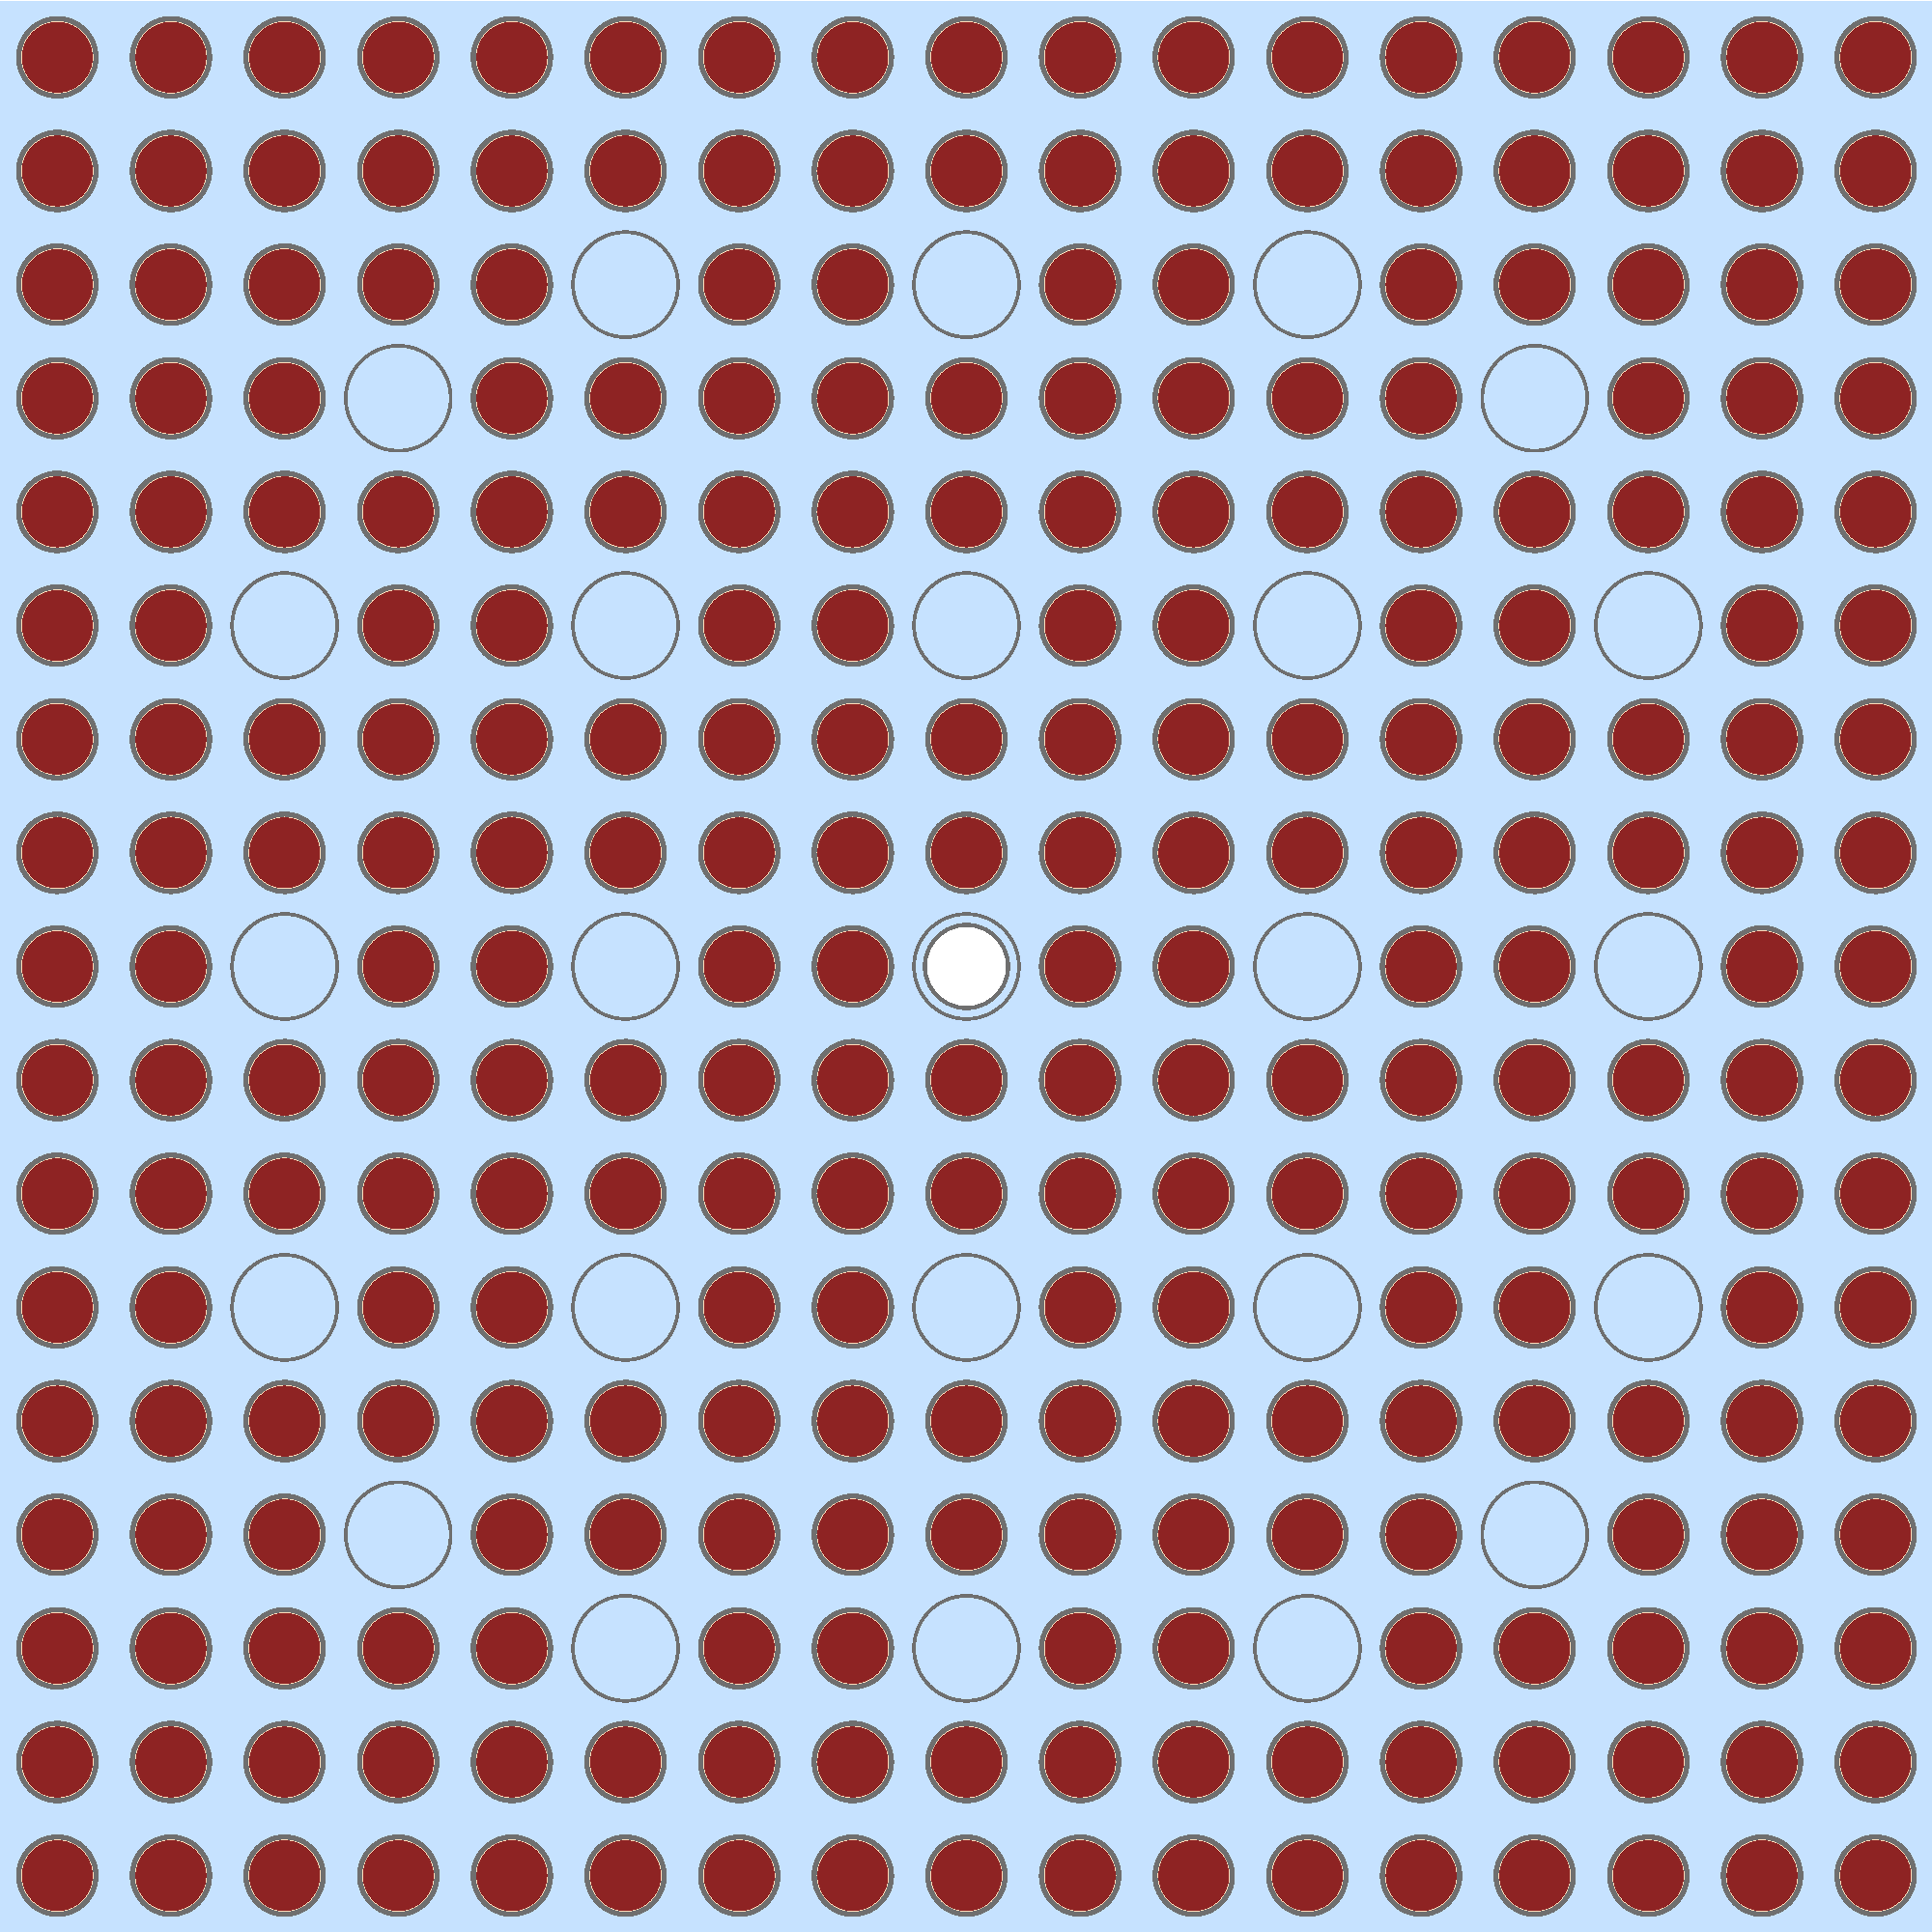
\includegraphics[width=0.8\linewidth]{figures/assembly/geometry}
  \caption{}
  \label{fig:null-assm}
\end{subfigure}
\begin{subfigure}{0.45\textwidth}
  \centering
  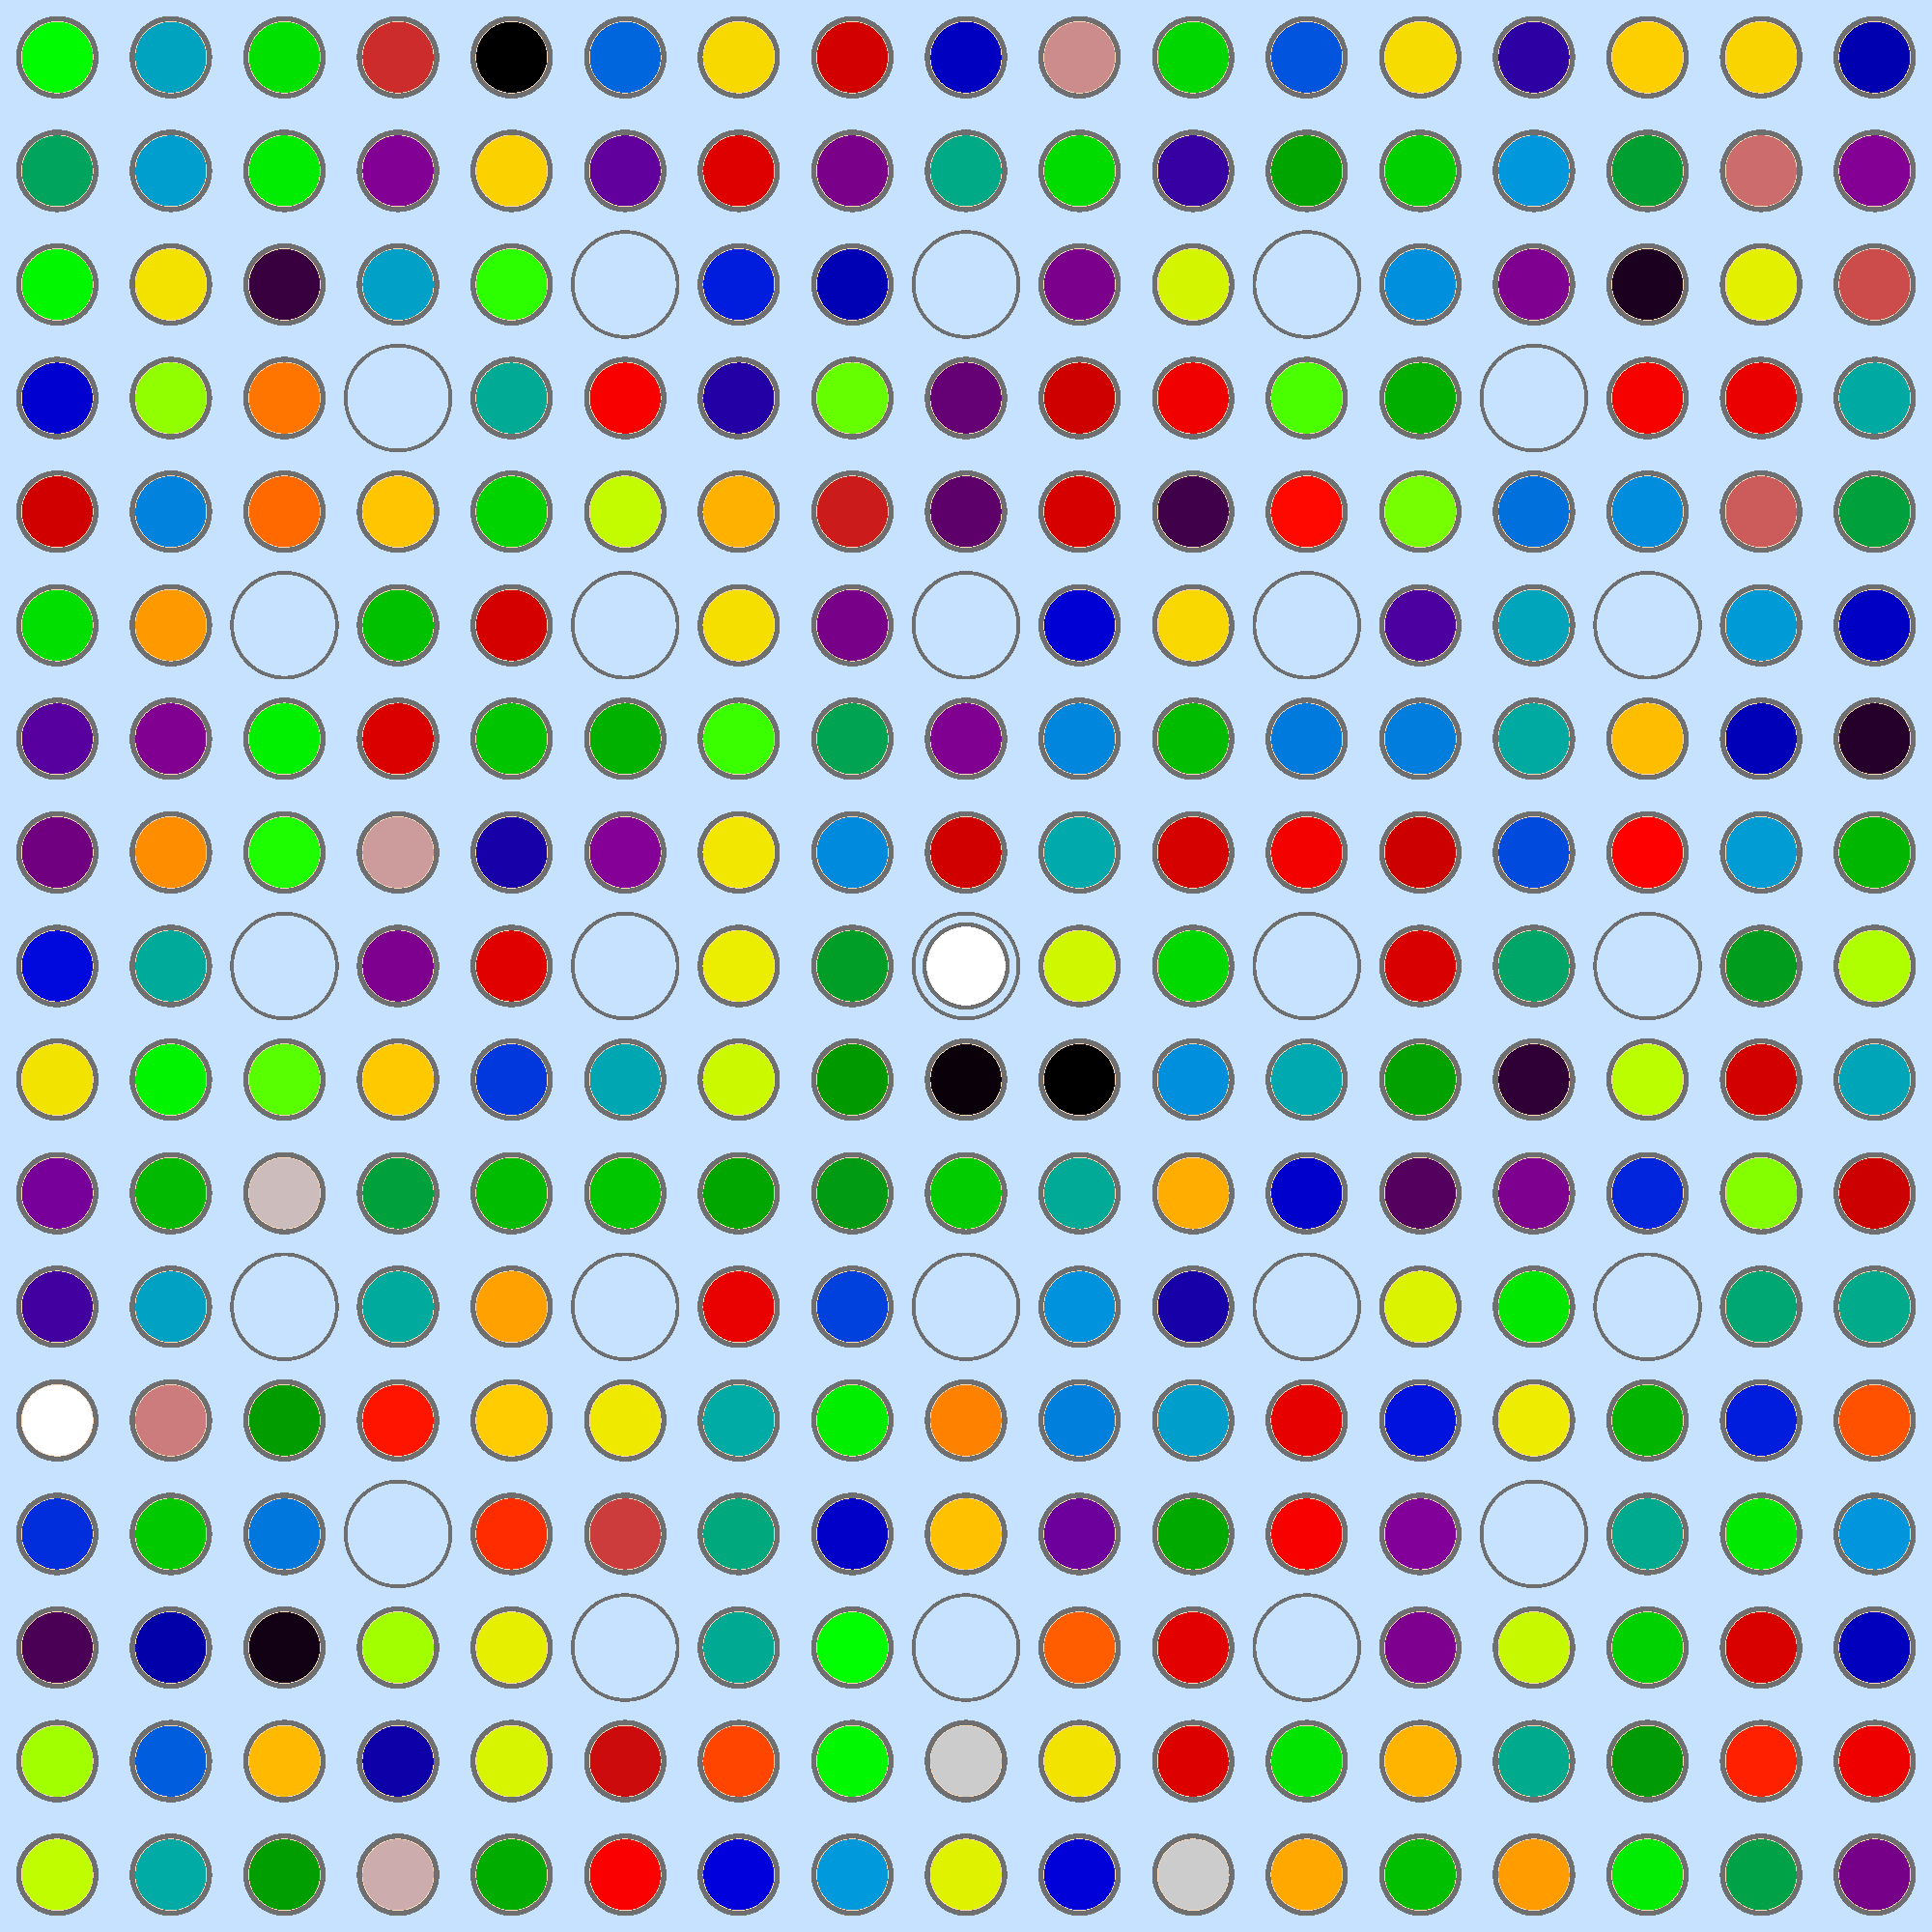
\includegraphics[width=0.8\linewidth]{figures/assembly/degenerate-materials}
  \caption{}
  \label{fig:degenerate-assm}
\end{subfigure}
\begin{subfigure}{0.45\textwidth}
  \centering
  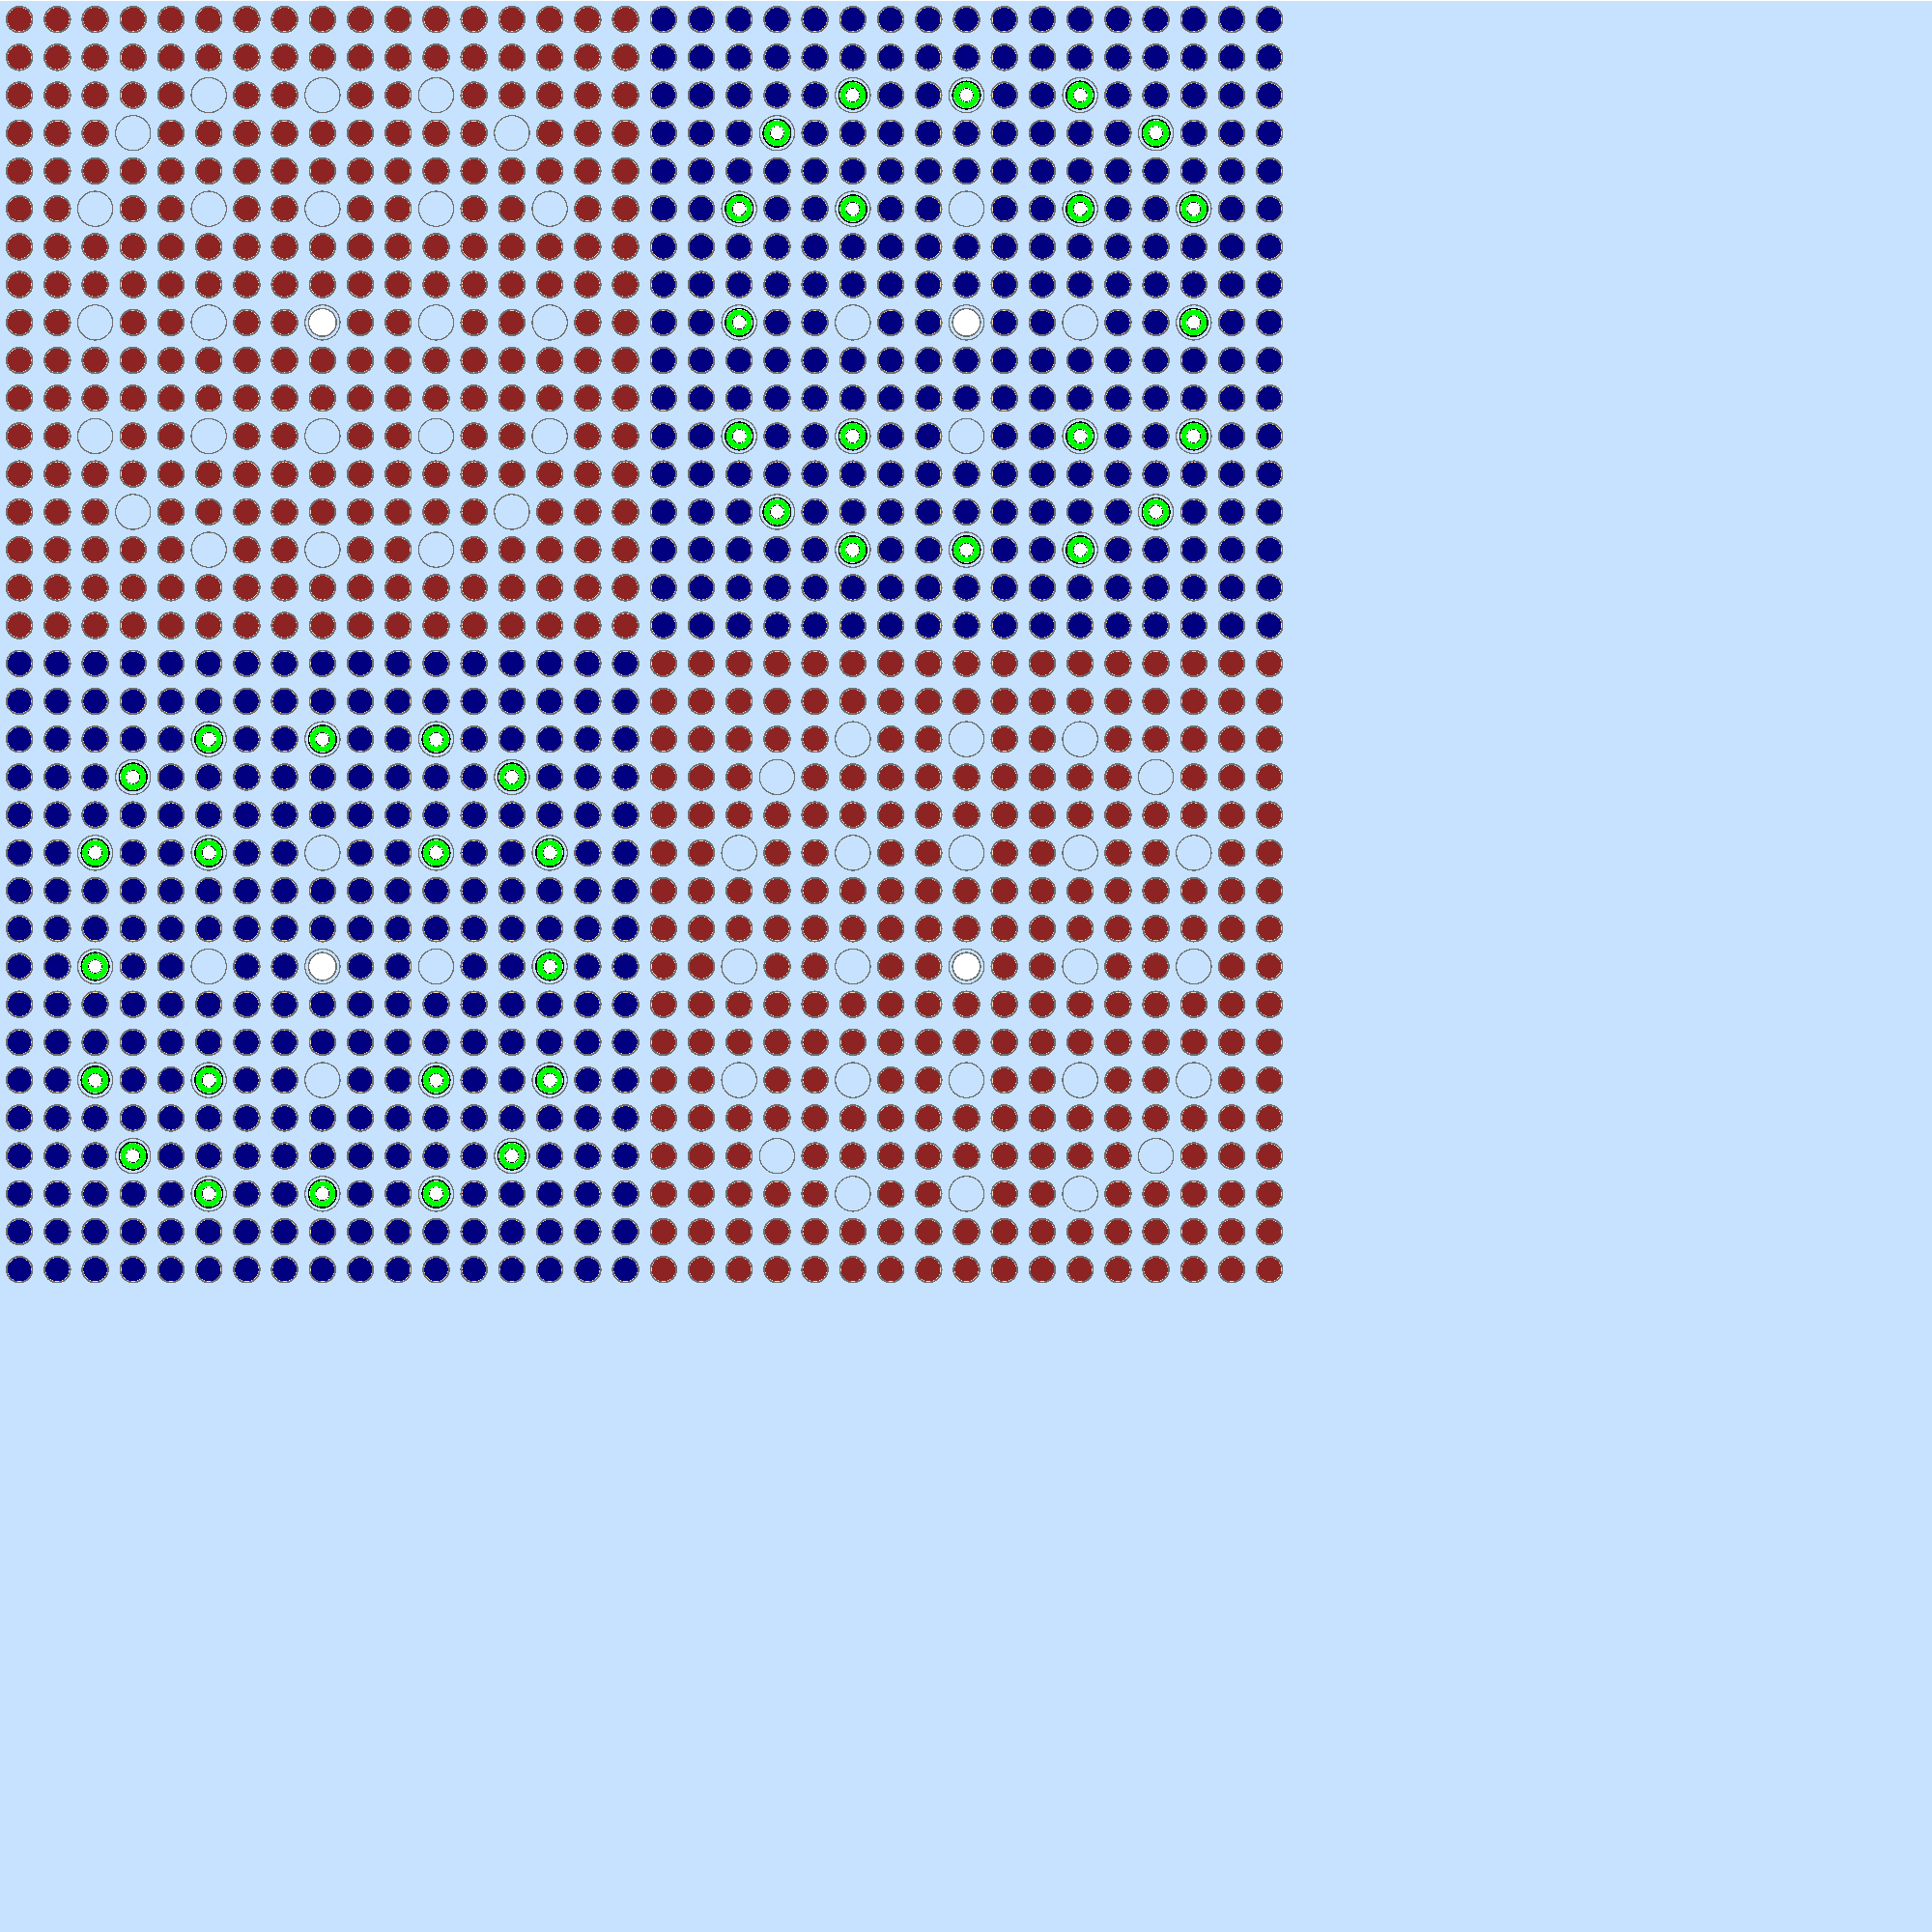
\includegraphics[width=0.8\linewidth]{figures/reflector/geometry}
  \caption{}
  \label{fig:null-reflector}
\end{subfigure}
\begin{subfigure}{0.45\textwidth}
  \centering
  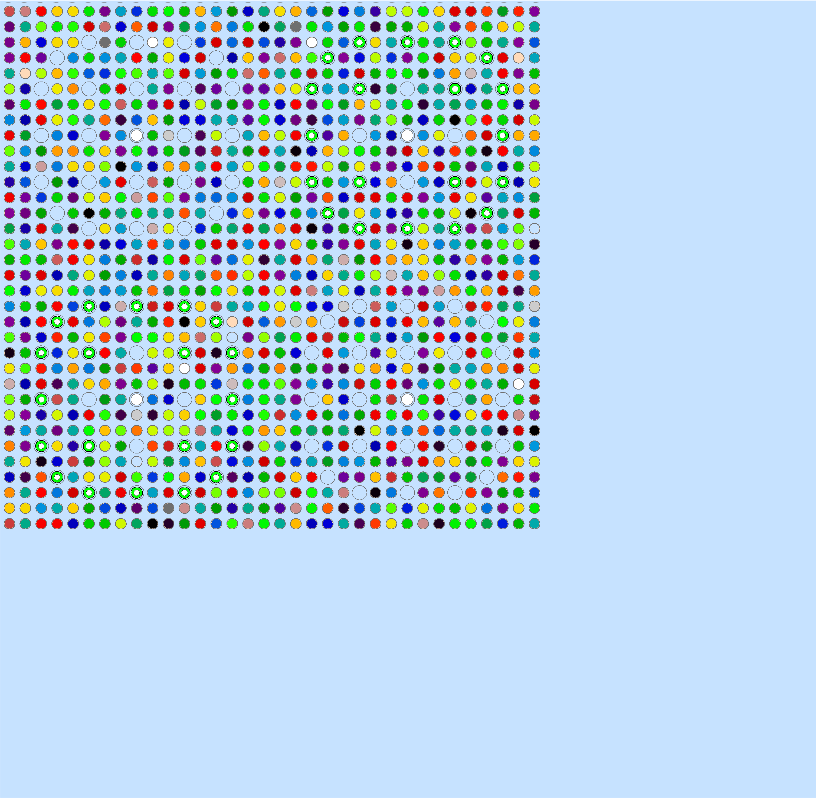
\includegraphics[width=0.8\linewidth]{figures/reflector/degenerate-materials}
  \caption{}
  \label{fig:degenerate-reflector}
\end{subfigure}
\caption{OpenMOC materials for the (a)-(b) assembly and (c)-(d) 2$\times$2 colorset models with null and degenerate homogenization, respectively.}
\label{fig:homogenization-schemes}
\end{figure*}

The \texttt{openmc.mgxs} module was used to compute 70-group MGXS with OpenMC for both the assembly and colorset benchmarks. The tallied MGXS data was condensed to coarse 2-group and 8-group structures with downstream data processing as necessary. The OpenMC simulations were performed with 1000 batches with 10$^{6}$ particle histories per batch for each benchmark. Stationarity of the fission source was obtained with 100 inactive batches for each benchmark. OpenMC's ``iso-in-lab'' feature was employed to enable consistent comparisons between OpenMC's reference results and OpenMOC's calculations with an isotropic in lab scattering source.

%%%%%%%%%%%%%%%%%%%%%%%%%%%%%%%%%%%%%%%%%%%%%%%%%%%%%%%%%%%%%%%%%%%%%%%%%%%%%%%
\subsubsection{Null Homogenization}
\label{subsubsec:homogenize-null}

The \textit{null} spatial homogenization scheme uses a single Monte Carlo calculation of the complete heterogeneous geometry to generate MGXS for each material. In this way, the null scheme fully abandons the multi-level approach used by most traditional approaches to generate MGXS. The spatially self-shielded flux is used to collapse the cross sections in each material with a unique isotopic composition. The null scheme does not account for spatial self-shielding effects experienced by different fuel pins filled by the same type of fuel, and instead averages these effects across the entire geometry. A single MGXS is employed in each instance of a material zone, such as a fuel pin replicated many times throughout a benchmark geometry.

%%%%%%%%%%%%%%%%%%%%%%%%%%%%%%%%%%%%%%%%%%%%%%%%%%%%%%%%%%%%%%%%%%%%%%%%%%%%%%%
\subsubsection{Degenerate Homogenization}
\label{subsubsec:homogenize-degenerate}

Unlike the null spatial homogenization scheme, the \textit{degenerate} scheme accounts for the different spatial self-shielding effects experienced by each instance of each fuel pin throughout a heterogeneous geometry. Like the null scheme, a single MC calculation of the complete heterogeneous geometry is used to generate MGXS for all materials. Unlike the null scheme, the MGXS are tallied separately for each instance of fissile material zones. For example, if a heterogeneous benchmark includes $N$ fuel pins, then $N$ collections of MGXS are separately tabulated for each fuel pin instance. The degenerate scheme tallies different MGXS even if the isotopic compositions in the fuel pin instances are identical (\textit{e.g.}, fresh fuel at the beginning of life) since each instance may experience different spatial self-shielding effects and hence have different MGXS.

The degenerate scheme generates MGXS for each fuel pin instance using OpenMC's distributed cell tallies~\citep{lax2014distribcell}. The OpenCG region differentiation algorithm~\citep{boyd2015opencg} is used to build a new OpenMOC geometry with unique cells and materials for each fuel pin. The MGXS are appropriately selected from OpenMC's distributed cell tallies to populate the MGXS in the OpenMOC materials. Multi-group transport calculations with MGXS generated using null and degenerate schemes may be compared to quantify the impact of modeling spatial self-shielding effects in MGXS for fissile zones in heterogeneous geometries.